\hypertarget{gracz_8cpp}{\section{Dokumentacja pliku /home/karolina/\-Pulpit/\-Project41\-Poker(1)/\-Project41\-Poker/\-Project41\-Poker/prj/src/gracz.cpp}
\label{gracz_8cpp}\index{/home/karolina/\-Pulpit/\-Project41\-Poker(1)/\-Project41\-Poker/\-Project41\-Poker/prj/src/gracz.\-cpp@{/home/karolina/\-Pulpit/\-Project41\-Poker(1)/\-Project41\-Poker/\-Project41\-Poker/prj/src/gracz.\-cpp}}
}


Definicja metody klasy \hyperlink{class_gracz}{Gracz}.  


{\ttfamily \#include $<$iostream$>$}\\*
{\ttfamily \#include \char`\"{}gracz.\-h\char`\"{}}\\*
Wykres zależności załączania dla gracz.\-cpp\-:\nopagebreak
\begin{figure}[H]
\begin{center}
\leavevmode
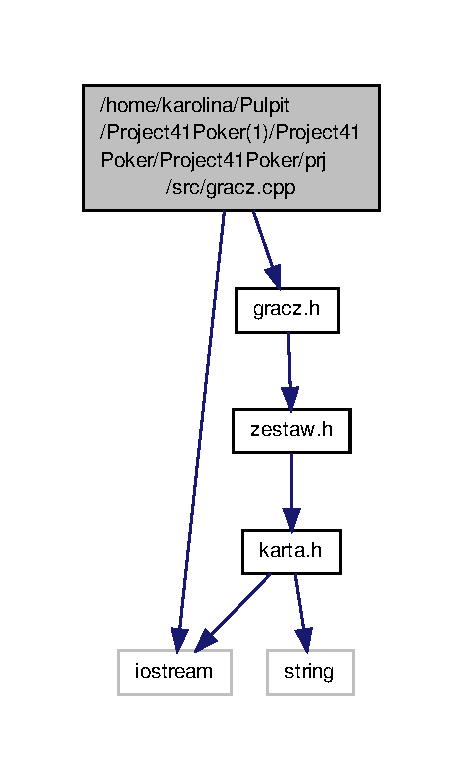
\includegraphics[width=222pt]{gracz_8cpp__incl}
\end{center}
\end{figure}


\subsection{Opis szczegółowy}
Zawiera definicjê metod klasy \hyperlink{class_gracz}{Gracz}. 

Definicja w pliku \hyperlink{gracz_8cpp_source}{gracz.\-cpp}.

